% Research deep dive -- code-backed literature 2025-2026.
%
% Build:  cd slides && make research_deep_dive.pdf
% Figures are generated from the committed harvest data; regenerate with
%   python3 slides/figures/make_figures.py --data research/data --out slides/figures

\documentclass[aspectratio=169,10pt]{beamer}
\usepackage{common/pdmtheme}
\graphicspath{{figures/}}

\title[Code-backed research 2025--2026]{Code-backed research, 2025--2026}
\subtitle{What the recent literature changes in the predictive-maintenance platform}
\author{Predictive Maintenance Platform}
\date{13 October 2026}

\begin{document}

% ---------------------------------------------------------------- title ----
\begin{frame}[plain]
  \vspace{6mm}
  {\LARGE\bfseries Code-backed research, 2025--2026}\\[2mm]
  {\large\color{pdmink2} What the recent literature changes in the platform}\par
  \vspace{5mm}\noindent{\color{pdmrule}\rule{\linewidth}{0.4pt}}\par
  \vspace{3mm}
  \begin{columns}[T]
    \begin{column}{0.46\textwidth}
      \scriptsize
      \kv{Window}{2025-01-01 to 2026-10-13}\\[1mm]
      \kv{Harvested}{1\,639 unique arXiv papers}\\[1mm]
      \kv{With resolvable code}{331}\\[1mm]
      \kv{After filtering}{\textbf{45}}\\[1mm]
      \kv{Reproduce}{\texttt{make research}}
    \end{column}
    \begin{column}{0.46\textwidth}
      \scriptsize\color{pdmink2}
      Every repository was resolved through the GitHub API on the generation
      date: it exists, and its licence, size, stars and last push are recorded
      as returned.\\[2mm]
      \textbf{No repository was executed.} ``Has code'' means the code exists,
      not that it reproduces the paper.
    \end{column}
  \end{columns}
  \srcnote{Branch \texttt{research/code-backed-deep-dive}. Tooling:
    \texttt{research/tools/harvest\_arxiv\_code.py}, \texttt{research/tools/curate.py}.
    Raw harvest committed under \texttt{research/data/}.}
\end{frame}

% --------------------------------------------------------------- question ---
\begin{frame}{The question, and why it is different from ``relevant papers''}
  \begin{columns}[T]
    \begin{column}{0.52\textwidth}
      The upstream \texttt{resources/academic\_papers.md} lists 32 papers chosen
      for \emph{relevance}. Right first filter, wrong question for a build team.
      \\[2mm]
      This asks something narrower and verifiable:
      \\[1.5mm]
      \begin{minipage}{\linewidth}
        \noindent{\color{pdmrule}\rule{\linewidth}{0.4pt}}\par\vspace{1mm}
        {\small\itshape Of the recent condition-monitoring literature, which
        papers come with code we can read, run and --- licence permitting ---
        reuse?}\par
        \vspace{1mm}\noindent{\color{pdmrule}\rule{\linewidth}{0.4pt}}
      \end{minipage}
      \\[2.5mm]
      That is a question about \emph{artefacts}, not ideas. It has an answer you
      can check.
    \end{column}
    \begin{column}{0.44\textwidth}
      \centering
      \hero{6.3\,\%}{of papers print a code URL\\in the abstract or comment}
      \\[4mm]
      \hero{27 / 45}{of the code-backed papers ship code\\with \emph{no usable licence}}
    \end{column}
  \end{columns}
  \takeaway{Relevance filters find ideas. Artefact filters find things you can
    build on this afternoon --- and most of them, legally, you cannot.}
\end{frame}

% ---------------------------------------------------------------- pipeline --
\begin{frame}{Pipeline}
  \centering
  \begin{tikzpicture}[node distance=5mm and 7mm]
    \node[pdmblk, minimum width=26mm] (q)   {22 arXiv queries\\\tiny 2025-01 to 2026-10};
    \node[pdmblk, minimum width=24mm, right=of q]  (uniq) {1\,639 unique\\papers};
    \node[pdmblk2, minimum width=26mm, right=of uniq] (abs) {103 with a code URL\\\tiny in abstract/comment};
    \node[pdmblk2, minimum width=26mm, below=of abs] (rev) {+239 via reverse\\\tiny GitHub README lookup};
    \node[pdmblk3, minimum width=24mm, right=of abs] (live) {331 repositories\\resolve};
    \node[pdmblkoff, minimum width=24mm, right=of live] (filt) {$-140$ aggregator\\$-146$ off-topic};
    \node[pdmblk3, minimum width=18mm, below=of filt] (keep) {\textbf{45 curated}};

    \draw[pdmarrow] (q) -- (uniq);
    \draw[pdmarrow] (uniq) -- (abs);
    \draw[pdmarrow] (uniq.south) |- (rev.west);
    \draw[pdmarrow] (abs) -- (live);
    \draw[pdmarrow] (rev.east) -| (live.south);
    \draw[pdmarrow] (live) -- (filt);
    \draw[pdmarrow] (filt) -- (keep);
    \begin{scope}[on background layer]
      \node[pdmgroup, fit=(abs)(rev), label={[pdmnote, anchor=north west]below left:
        {\tiny code discovery}}] {};
    \end{scope}
  \end{tikzpicture}
  \\[1.5mm]
  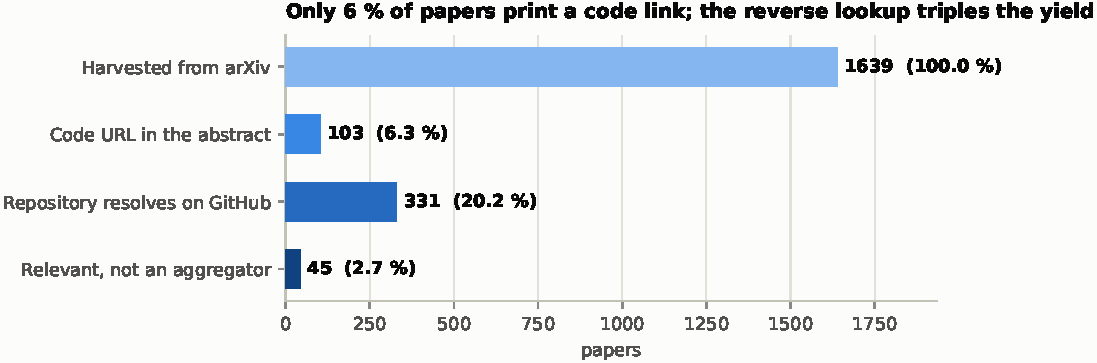
\includegraphics[width=0.64\linewidth]{fig_funnel.pdf}
  \srcnote{Reverse lookup: \nolinkurl{GET /search/repositories?q="<arxiv_id>"+in:readme} ---
    900 searches spent, 239 matched (27\,\%), capped at 30 requests/minute even authenticated.}
\end{frame}

% --------------------------------------------------------- the filter bug ---
\begin{frame}{The filter that the first version of this needed}
  \begin{columns}[T]
    \begin{column}{0.5\textwidth}
      \small
      The reverse lookup over-reports in one systematic way, and the first run
      was visibly wrong because of it.
      \\[2mm]
      A whole class of repositories --- \texttt{*-arxiv-daily},
      \texttt{awesome-*}, paper lists --- cites \emph{thousands} of arXiv IDs in
      its README.
      \\[2mm]
      The first run therefore ranked:
      \\[1mm]
      \scriptsize
      $\bullet$ \gh{BaiShuanghao/my_arXiv_daily} (217$\star$) as the code for
      \textbf{eight} unrelated papers\\[1mm]
      $\bullet$ \gh{halsay/ASR-TTS-paper-daily} (513$\star$) as the code for a
      paper on analog resonant networks
    \end{column}
    \begin{column}{0.46\textwidth}
      \small
      Two filters remove them:
      \\[2mm]
      \textbf{1. Name and description patterns} ---
      \texttt{arxiv-daily}, \texttt{paper-daily}, \texttt{awesome-},
      \texttt{\^{}arxiv-}, \texttt{*-list}, \texttt{literature}.
      \\[2mm]
      \textbf{2. The robust one:} any repository cited by $\ge 3$ different
      papers through README search. Real code is cited by one paper, sometimes
      two when a lab reuses a repository. Three is already an aggregator.
      \\[2.5mm]
      \scriptsize\color{pdmink2}
      54 repositories dropped $\Rightarrow$ 140 papers whose only ``code'' was
      a listing.
    \end{column}
  \end{columns}
  \takeaway{An automated literature harvest needs an adversarial filter, and the
    data-driven signal (how many papers does this repo claim?) beats the
    pattern match.}
\end{frame}

% ------------------------------------------------------------ where it is ---
\begin{frame}{Where the code-backed work actually is}
  \begin{columns}[T]
    \begin{column}{0.56\textwidth}
      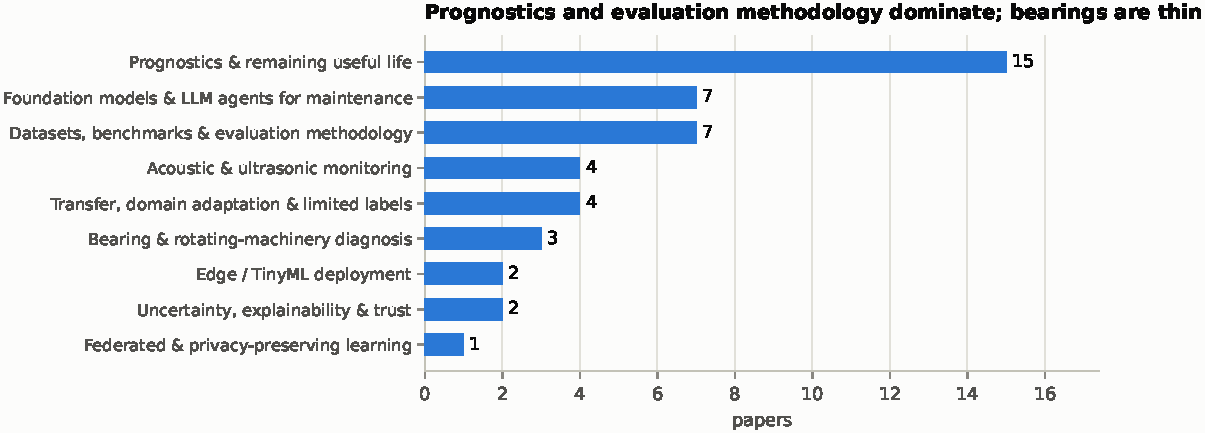
\includegraphics[width=\linewidth]{fig_themes.pdf}
    \end{column}
    \begin{column}{0.41\textwidth}
      \small
      Two things stand out, and both are uncomfortable.
      \\[2mm]
      \textbf{Prognostics and evaluation methodology dominate.} The field is
      arguing about \emph{how it measures}, not which architecture wins.
      \\[2mm]
      \textbf{Bearings are thin} --- 3 of 45. The serious rotating-machinery
      literature is in \emph{MSSP}, \emph{IEEE TIM} and the PHM Society
      conferences, which are not on arXiv and do not ship code.
      \\[2mm]
      \textbf{Acoustic emission: zero.} Not one code-backed AE paper in
      21 months.
    \end{column}
  \end{columns}
  \takeaway{This list is biased toward the ML-facing half of the field. Know
    that before using it to plan hardware.}
\end{frame}

% ----------------------------------------------------------- shift 1: leak --
\begin{frame}{Shift 1 --- evaluation methodology became the finding}
  \begin{columns}[T]
    \begin{column}{0.48\textwidth}
      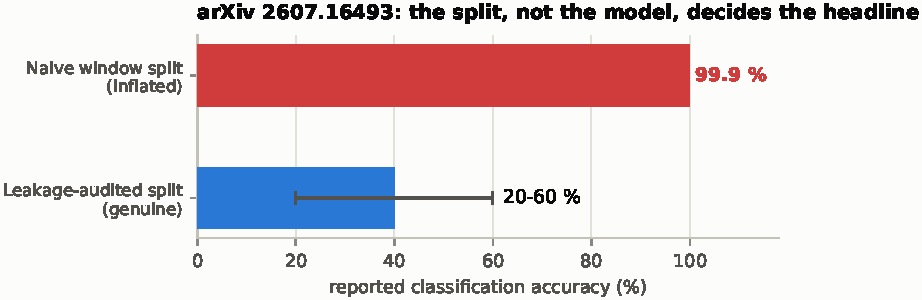
\includegraphics[width=\linewidth]{fig_leakage.pdf}
      \\[1mm]
      \scriptsize
      \arx{2607.16493} (CALIBRA, MIT) on C-MAPSS, NASA IMS and UCI Hydraulic:
      naive sliding-window splitting inflates accuracy \textbf{from a genuine
      20--60\,\% to 99.9\,\%} --- or collapses it to 0\,\% through degenerate
      class representation.
    \end{column}
    \begin{column}{0.48\textwidth}
      \small
      It is a cluster, not one corrective paper:
      \\[1.5mm]
      \scriptsize
      \arx{2605.28345} \textbf{Picid} (EPFL-IMOS) --- evaluation
      \emph{infrastructure} that enforces leakage-safe, deterministic dataset
      construction. A lab thought this was worth building.
      \\[1.5mm]
      \arx{2607.08273} --- bearing RUL with held-out units defined by
      \textbf{load--speed regime}, reporting nMAE 0.1477 \emph{with} empirical
      90\,\% interval coverage.
      \\[1.5mm]
      \arx{2606.29339} --- separates \textbf{sensor-failure tolerance} from
      \textbf{low-SNR robustness}, two things routinely conflated, over Hi-net
      seismic + FORGE borehole DAS + MAFAULDA vibration.
    \end{column}
  \end{columns}
  \takeaway{The gap between a leaked and an honest split is larger than the gap
    between any two architectures in this window. Protocol discipline buys more
    than model selection.}
\end{frame}

% --------------------------------------------------------- shift 2: tsfm ----
\begin{frame}{Shift 2 --- foundation models became a frozen feature extractor}
  \centering
  \begin{tikzpicture}[node distance=4mm and 9mm]
    \node[pdmblk, minimum width=22mm] (f)  {63-float feature\\frames};
    \node[pdmblk3, minimum width=30mm, right=of f] (b) {\textbf{frozen} time-series\\foundation model};
    \node[pdmblk2, minimum width=24mm, right=of b] (h) {small head\\\tiny $\sim$10\,k params};
    \node[pdmblk, minimum width=20mm, right=of h] (o) {fault class\\or RUL};
    \draw[pdmarrow] (f) -- (b); \draw[pdmarrow] (b) -- (h); \draw[pdmarrow] (h) -- (o);
    \node[pdmnote, below=1.5mm of b] {no gradient flows here};
    \node[pdmnote, below=1.5mm of h] {the only thing trained};
  \end{tikzpicture}
  \\[3mm]
  \begin{columns}[T]
    \begin{column}{0.48\textwidth}
      \scriptsize
      \arx{2606.11990} (EUSIPCO 2026) --- \textbf{Chronos-2 frozen} + a small
      regression head consistently beats recurrent baselines on real industrial
      sensor data, with no feature engineering and no large labelled set.
      \\[1.5mm]
      \arx{2601.22631} \textbf{PEFT-MuTS} --- few-shot RUL via
      parameter-efficient fine-tuning, and explicitly ``contrary to the widely
      held view'': transfer does \emph{not} need similar devices.
      \\[1.5mm]
      \arx{2604.20122} --- adaptive conformal anomaly detection on
      \gh{ibm-granite/granite-tsfm} (910$\star$, Apache-2.0) --- maintained,
      permissive infrastructure rather than a research dump.
    \end{column}
    \begin{column}{0.48\textwidth}
      \small\textbf{What we are assuming, stated plainly}
      \\[1.5mm]
      \scriptsize
      The backbone consumes our \emph{feature frames} at one frame per
      acquisition --- \textbf{not} 25.6\,kHz waveforms. No paper in this window
      demonstrates a TSFM on raw high-rate vibration.
      \\[2mm]
      It does \textbf{not} replace the unsupervised path: a frozen backbone
      still needs labels for its head, and a new site has none. This is a
      Phase-2 capability, behind the unsupervised-first commitment.
    \end{column}
  \end{columns}
\end{frame}

% ------------------------------------------------- shifts 3-5 (condensed) ---
\begin{frame}{Shifts 3--5}
  \small
  \begin{columns}[T]
    \begin{column}{0.31\textwidth}
      \textbf{3. Calibration is standard now}
      \\[1.5mm]
      \scriptsize
      $\bullet$ \arx{2607.08273} forms RUL intervals by empirical residual
      calibration and reports \emph{coverage}, not just MAE.\\[1mm]
      $\bullet$ \arx{2604.20122} applies adaptive conformal prediction ---
      distribution-free coverage that survives drift.\\[1mm]
      $\bullet$ \arx{2511.12240} \textbf{SCI} wraps a model in a closed
      entropy-gated loop: stop, continue, or escalate.\\[1mm]
      $\bullet$ \arx{2606.12486} (Scania) builds on wear being
      \textbf{monotonically non-decreasing} --- a physics prior that doubles as
      a calibration check.
    \end{column}
    \begin{column}{0.31\textwidth}
      \textbf{4. INT4 is defensible}
      \\[1.5mm]
      \scriptsize
      \arx{2604.08474}: a 9\,697-parameter 1-D CNN, federated on C-MAPSS,
      quantised at 32/8/4/2 bits over \textbf{10 seeds}.
      \\[1.5mm]
      INT4 is \textbf{statistically indistinguishable} from FP32
      ($p=0.341$ FD001, $p=0.264$ MAE FD002) at $8\times$ reduction.
      \\[1.5mm]
      Multi-seed with p-values is more rigorous than this literature's norm,
      and the model size matches ours (Deep SVDD $\approx$1.7\,k params).
      \\[1.5mm]
      \arx{2606.24173} keeps \emph{classical} baselines in the table alongside
      accuracy, size and CPU latency. Right shape for our per-kit tables.
    \end{column}
    \begin{column}{0.31\textwidth}
      \textbf{5. Adaptation went source-free}
      \\[1.5mm]
      \scriptsize
      Both shifts driven by one constraint: \emph{you cannot move the data}.
      \\[1.5mm]
      \arx{2503.08749} \textbf{SDALR} (41$\star$) --- adapt a bearing model to a
      new domain with \textbf{no access to source data}. Lets customer A's model
      serve customer B without either's data leaving site.
      \\[1.5mm]
      \arx{2609.35792} --- \textbf{matched-protocol} comparison of ring gossip
      vs FedAvg vs local vs centralised: one implementation, architecture,
      split and budget. Removes the aggregation server entirely.
    \end{column}
  \end{columns}
  \takeaway{Source-free adaptation across tenants; federation or gossip within a
    tenant. ``Customer data never joins another customer's training round'' is a
    far easier claim to defend for FedRAMP.}
\end{frame}

% ------------------------------------------------------------- the licence --
\begin{frame}{The constraint nobody mentions in a literature review}
  \begin{columns}[T]
    \begin{column}{0.54\textwidth}
      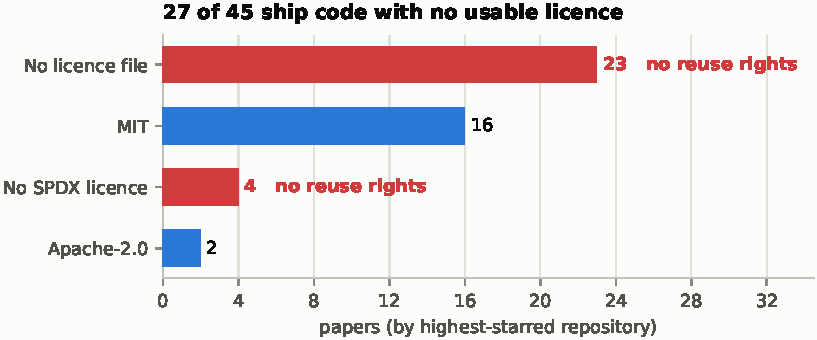
\includegraphics[width=\linewidth]{fig_licence.pdf}
      \\[1mm]
      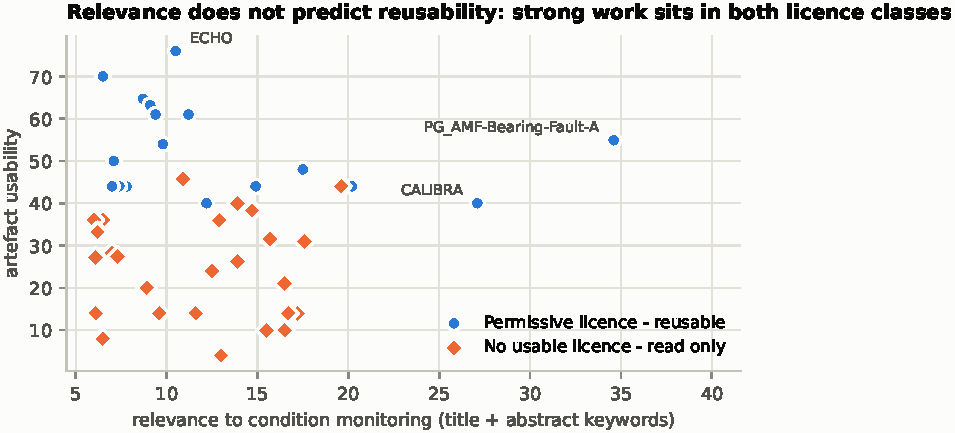
\includegraphics[width=\linewidth]{fig_usability.pdf}
    \end{column}
    \begin{column}{0.43\textwidth}
      \small
      A public GitHub repository with no \texttt{LICENSE} file is
      \textbf{all rights reserved}. You may read it and learn the method. You
      may not copy a function out of it.
      \\[2mm]
      And the most \emph{useful} repositories here are frequently the
      unusable ones:
      \\[1.5mm]
      \scriptsize
      $\bullet$ \gh{BdLab405/SDALR} (41$\star$, the best-regarded on-topic
      bearing repo in the window) --- \textbf{no licence}\\[1mm]
      $\bullet$ \gh{EPFL-IMOS/picid} (the evaluation infrastructure we most want)
      --- \textbf{NOASSERTION}
      \\[2.5mm]
      \small\textbf{Mitigation that actually works:} open an issue asking for a
      licence. Most academic authors intend reuse and simply did not add the
      file. Costs an issue and a week.
    \end{column}
  \end{columns}
\end{frame}

% ----------------------------------------------------------- what to do -----
\begin{frame}{Adopt now --- permissive, relevant, substantial}
  \scriptsize
  \begin{tabular}{@{}p{0.27\linewidth}p{0.11\linewidth}p{0.555\linewidth}@{}}
    \toprule
    \textbf{Repository} & \textbf{Licence} & \textbf{What we take, and why} \\
    \midrule
    \ghs{nbbllxx0/Empirical-Calibration-and-Conditional-Reliability-Diagnostics}%
      {nbbllxx0/Empirical-Calibration-\dots}
      & MIT & \textbf{Highest-priority read of the list.} Closest paper to our
        actual problem: bearings, time-varying load and speed, 10 documented
        units, calibrated intervals. Take the regime-based split and the
        empirical residual calibration. \\[1mm]
    \gh{therealdeadbeef/aerospace-fl-quantization}
      & MIT & The multi-seed quantisation protocol, not the model. Makes every
        per-kit INT8/INT4 claim defensible. \\[1mm]
    \gh{ISAO9/cephalon-v2}
      & MIT & Two-axis robustness test design: channel dropout and SNR
        degradation as \emph{separate} reported conditions. We have no
        sensor-failure test at all today. \\[1mm]
    \gh{rajeevfee/PG_AMF-Bearing-Fault-Analysis-}
      & MIT & Learned adaptive moment features vs our 14 fixed time-domain
        indicators. Parameters are flash constants either way --- no runtime
        penalty if it wins. \\[1mm]
    \gh{TakuyaFujimura/dcase-asd-toolkit}
      & MIT & Reference implementation for the acoustic channel; a toolkit, not
        a one-paper dump. \\[1mm]
    \gh{ZhixiangWang-CN/gossip-lstm-cmapss}
      & MIT & The matched-protocol harness. The only honest way to decide
        federated-vs-alternatives. \\[1mm]
    \gh{ibm-granite/granite-tsfm}
      & Apache-2.0 & Adaptive conformal thresholds --- replaces our parametric
        Gumbel tail extrapolation. \\
    \bottomrule
  \end{tabular}
  \srcnote{Full triage with sequencing and costs:
    \texttt{research/deep\_dive/03\_adoption\_shortlist.md}.
    Licences as returned by the GitHub API on 2026-10-13 --- re-check before
    copying anything.}
\end{frame}

% ------------------------------------------------------------- plan deltas --
\begin{frame}{What this changes in the seven product plans}
  \scriptsize
  \begin{tabular}{@{}p{0.2\linewidth}p{0.075\linewidth}p{0.615\linewidth}@{}}
    \toprule
    \textbf{Plan} & \textbf{Severity} & \textbf{Change} \\
    \midrule
    00 Overview & \textcolor{pdmcrit}{\textbf{High}} &
      Evaluation protocol becomes a phase-\emph{exit gate}: named split, zero
      leakage violations, regime-level held-out units, the two robustness axes
      reported separately, metrics quoted at an agreed alarm budget. \\[0.8mm]
    01 Sensor HW & Medium &
      Keep AE as the hardware differentiator and keep the front-end on the PCB,
      but move AE \emph{algorithms} out of v1: zero code-backed AE papers and no
      public AE benchmark to validate against. Ship the 6\,kHz MEMS path first. \\[0.8mm]
    02 Edge firmware & Medium &
      Add an INT4 evaluation path. Replace schedule-driven tiering with
      \emph{uncertainty-gated} escalation (cheap indicators $\to$ spectrum $\to$
      envelope $\to$ raw snapshot). \\[0.8mm]
    03 IoT pipeline & --- &
      No architectural change. Add per-device sequence-gap accounting: a sensor
      dropping 30\,\% of frames looks healthy on a trend chart. \\[0.8mm]
    04 ML/AI engine & \textcolor{pdmcrit}{\textbf{High}} &
      Frozen-TSFM + small head as a Phase-2 track. Conformal intervals replace
      parametric tail extrapolation. Enforce monotonicity on the health index. \\[0.8mm]
    05 Cloud platform & Medium &
      Source-free adaptation across tenants; federation or gossip within a
      tenant. \\[0.8mm]
    06 CMMS dashboard & Medium &
      Abstention and calibrated confidence become first-class UI states. RUL
      renders as a distribution, never a point. \\[0.8mm]
    07 Electrical & Low &
      One code-backed MCSA paper in 21 months. Keep the plan, lower the stated
      confidence, budget for an \emph{own} measurement campaign rather than
      literature transfer. \\
    \bottomrule
  \end{tabular}
  \srcnote{Full reasoning per plan: \texttt{research/deep\_dive/02\_gap\_analysis\_vs\_plans.md}.}
\end{frame}

% ---------------------------------------------------------------- not do ----
\begin{frame}{Three things not to do, and what did not change}
  \begin{columns}[T]
    \begin{column}{0.48\textwidth}
      \small\textbf{Do not}
      \\[1.5mm]
      \scriptsize
      \textbf{1. Benchmark on C-MAPSS.} Nine of 45 entries use it. Simulated
      turbofan, no vibration channel, saturated. It would make our results
      comparable to the literature and uninformative about the product.
      \\[1.5mm]
      \textbf{2. Vendor unlicensed code.} 27 of 45. Read them; do not copy them.
      \\[1.5mm]
      \textbf{3. Chase architecture.} The leaked-vs-honest split gap
      (99.9\,\% vs 20--60\,\%) exceeds any architecture gap in this window.
    \end{column}
    \begin{column}{0.48\textwidth}
      \small\textbf{What did not change}
      \\[1.5mm]
      \scriptsize
      $\bullet$ \textbf{Envelope analysis and spectral kurtosis remain the
      technique of record} for bearing faults. Nothing displaces them;
      \arx{2606.26317} generalises adaptive moments but works inside exactly
      that framework.
      \\[1mm]
      $\bullet$ \textbf{Unsupervised one-class detection is still the only
      day-one option.} No paper here gets around the absence of labelled
      failures at a new site.
      \\[1mm]
      $\bullet$ \textbf{Nobody solved cross-machine generalisation.}
      Source-free adaptation, PEFT and TSFM embeddings all \emph{reduce} the
      target data needed. None removes it.
      \\[1mm]
      $\bullet$ \textbf{The gap that matters is data, not method:} no public
      dataset covers a wireless MEMS sensor on a real industrial machine over a
      multi-month degradation. That is our pilot, and it is on the critical
      path.
    \end{column}
  \end{columns}
\end{frame}

% ---------------------------------------------------------------- method ----
\begin{frame}[fragile]{Reproducing this}
\begin{lstlisting}[language=bash]
# ~45 min: 22 arXiv queries, 103 repo lookups, 900 README searches.
# Standard library only -- runs in CI and on a gateway, no virtualenv.
GITHUB_TOKEN=<public-read> python3 research/tools/harvest_arxiv_code.py \
    --out research/data/harvest_$(date +%Y%m%d).json \
    --from 2025-01-01 --max-per-topic 150 --readme-search-budget 900

python3 research/tools/curate.py --in research/data/harvest_$(date +%Y%m%d).json \
    --out-md research/code_backed_papers_2025_2026.md \
    --out-csv research/data/papers_with_code.csv \
    --out-json research/data/curated.json

python3 slides/figures/make_figures.py   # figures come from the committed data
\end{lstlisting}
  \scriptsize
  \textbf{Limitations, stated up front.} arXiv only --- \emph{MSSP}, \emph{IEEE TIM}
  and the PHM Society conferences carry much of the serious condition-monitoring
  literature and are absent. English abstracts only. README-search recall is
  bounded by GitHub's indexing. A single snapshot: star counts and push dates
  aged the moment it ran. The relevance threshold (6.0) was calibrated by hand
  against this harvest, and both failure directions are recorded with examples
  in the audit trail of the generated list, so it can be re-argued rather than
  taken on trust.
\end{frame}

\end{document}
